% Options for packages loaded elsewhere
\PassOptionsToPackage{unicode}{hyperref}
\PassOptionsToPackage{hyphens}{url}
%
\documentclass[
  11pt,
  a4paper,
]{article}
\usepackage{amsmath,amssymb}
\usepackage{lmodern}
\usepackage{iftex}
\ifPDFTeX
  \usepackage[T1]{fontenc}
  \usepackage[utf8]{inputenc}
  \usepackage{textcomp} % provide euro and other symbols
\else % if luatex or xetex
  \ifXeTeX
    \usepackage{zxjatype} 
    \usepackage[ipaex]{zxjafont}
    \setromanfont{Times New Roman}
  \fi
  \usepackage{unicode-math}
  \defaultfontfeatures{Scale=MatchLowercase}
  \defaultfontfeatures[\rmfamily]{Ligatures=TeX,Scale=1}
\fi
% Use upquote if available, for straight quotes in verbatim environments
\IfFileExists{upquote.sty}{\usepackage{upquote}}{}
\IfFileExists{microtype.sty}{% use microtype if available
  \usepackage[]{microtype}
  \UseMicrotypeSet[protrusion]{basicmath} % disable protrusion for tt fonts
}{}
\usepackage{xcolor}
\IfFileExists{xurl.sty}{\usepackage{xurl}}{} % add URL line breaks if available
\IfFileExists{bookmark.sty}{\usepackage{bookmark}}{\usepackage{hyperref}}
\hypersetup{
  pdftitle={Charitable Giving, Tax Reform, and Self-selection of Tax Relief: Evidence from South Korea},
  hidelinks,
  pdfcreator={LaTeX via pandoc}}
\urlstyle{same} % disable monospaced font for URLs
\usepackage[left=3cm,right=3cm,top=3cm,bottom=3cm]{geometry}

\usepackage{setspace}
\renewcommand{\baselinestretch}{1.5}
\usepackage{float}

\usepackage{longtable,booktabs,array}
\usepackage{threeparttable, threeparttablex, multirow}
\usepackage{calc} % for calculating minipage widths
% Correct order of tables after \paragraph or \subparagraph
\usepackage{etoolbox}
\makeatletter
\patchcmd\longtable{\par}{\if@noskipsec\mbox{}\fi\par}{}{}
\makeatother
% Allow footnotes in longtable head/foot
\IfFileExists{footnotehyper.sty}{\usepackage{footnotehyper}}{\usepackage{footnote}}
\makesavenoteenv{longtable}
\usepackage{graphicx}
\makeatletter
\def\maxwidth{\ifdim\Gin@nat@width>\linewidth\linewidth\else\Gin@nat@width\fi}
\def\maxheight{\ifdim\Gin@nat@height>\textheight\textheight\else\Gin@nat@height\fi}
\makeatother
% Scale images if necessary, so that they will not overflow the page
% margins by default, and it is still possible to overwrite the defaults
% using explicit options in \includegraphics[width, height, ...]{}
\setkeys{Gin}{width=\maxwidth,height=\maxheight,keepaspectratio}
% Set default figure placement to htbp
\makeatletter
\def\fps@figure{htbp}
\makeatother
\setlength{\emergencystretch}{3em} % prevent overfull lines
\providecommand{\tightlist}{%
  \setlength{\itemsep}{0pt}\setlength{\parskip}{0pt}}
\setcounter{secnumdepth}{5}
\newlength{\cslhangindent}
\setlength{\cslhangindent}{1.5em}
\newlength{\csllabelwidth}
\setlength{\csllabelwidth}{3em}
\newlength{\cslentryspacingunit} % times entry-spacing
\setlength{\cslentryspacingunit}{\parskip}
\newenvironment{CSLReferences}[2] % #1 hanging-ident, #2 entry spacing
 {% don't indent paragraphs
  \setlength{\parindent}{0pt}
  % turn on hanging indent if param 1 is 1
  \ifodd #1
  \let\oldpar\par
  \def\par{\hangindent=\cslhangindent\oldpar}
  \fi
  % set entry spacing
  \setlength{\parskip}{#2\cslentryspacingunit}
 }%
 {}
\usepackage{calc}
\newcommand{\CSLBlock}[1]{#1\hfill\break}
\newcommand{\CSLLeftMargin}[1]{\parbox[t]{\csllabelwidth}{#1}}
\newcommand{\CSLRightInline}[1]{\parbox[t]{\linewidth - \csllabelwidth}{#1}\break}
\newcommand{\CSLIndent}[1]{\hspace{\cslhangindent}#1}


\ifLuaTeX
  \usepackage{selnolig}  % disable illegal ligatures
\fi

\makeatletter
\def\@fnsymbol#1{\ensuremath{\ifcase#1\or \dagger\or \ddagger\or
   \mathsection\or \mathparagraph\or \|\or **\or \dagger\dagger
   \or \ddagger\ddagger \else\@ctrerr\fi}}
    \makeatother
\title{Charitable Giving, Tax Reform, and Self-selection of Tax Relief: Evidence from South Korea  }
\author{
    Hiroki Kato
  \thanks{Graduate School of Economics, Osaka University, Japan. E-mail: vge008kh@stundent.econ.osaka-u.ac.jp  }
  \and
    Tsuyoshi Goto
  \thanks{Graduate School of Social Sciences, Chiba University, Japan. E-mail: t.goto@chiba-u.jp  }
  \and
    Youngrok Kim
  \thanks{Graduate School of Economics, Kobe University, Japan.  }
  \and
  }

\date{2021/11/14}


\begin{document}
\begin{spacing}{1}
  \maketitle
\end{spacing}
\begin{spacing}{1}
  \begin{abstract}
    This paper investigates the price elasticity of charitable giving utilizing South Korean tax reform in 2014, when the tax relief on charitable giving changed from tax deduction to tax credit. Although many research on the price elasticity of charitable giving use tax return data or ignore declaration cost for charitable giving to receive tax relief, this paper uses a survey panel data and considers the existence of declaration cost for tax reliefs on charitable giving.
    By considering the declaration of charitable giving and exploiting the different declaration cost between wage earners and self-employed workers as instrument variable (IV), we estimate the giving price elasticity on the donation. As a result, we find that the estimation about the price elasticity is -1.5 \(\sim\) -1.8 in terms of intensive margins.
    Moreover, our estimation suggest that the price elasticity for the extensive margins is less than -1.8, which is much less than the estimates of extant research.
    
            \noindent
    \textbf{Key words}: Charitable giving, Giving price, Tax reform, South Korea
        
        \noindent
    \textbf{JEL Codes}: D91, I10, I18
        
  \end{abstract}
\end{spacing}

\hypertarget{introduction}{%
\section{Introduction}\label{introduction}}

In many countries, governments set a tax relief for charitable giving. This is because, if subsidizing charitable giving induces a large increase in donations, it is desirable for public good provision. As Saez (2004) shows, it is known that the price elasticity of charitable donations is a key parameter to evaluate the welfare implication. To evaluate the effect of tax relief, many empirical papers investigate the elasticity of charitable donations with respect to their tax price and find that the price elasticity is around -1 in terms of intensive margin, using the data from tax record (Almunia et al., 2020; Auten et al., 2002; Bakija and Heim, 2011; Fack and Landais, 2010; Randolph, 1995).

However, there are two issues of the estimation as for the declaration of tax and charitable giving.
First issue is about the sample selection. Most of the analysis based on tax record only captures the effect for tax filers, while charitable donation may also be conducted by those who do not declare their tax. Thus, as some papers such as Rehavi and Shack (2013) and Backus and Grant (2019) point out, the estimation based on the tax return data will contain the sample selection bias.

Second issue is that the declaration for charitable giving (not the declaration of tax) is endogenous to the price of charitable giving. This is because the declaration for charitable giving is required to apply for the tax relief on charitable giving, and the effect of giving price on the amount of giving may represent the difference of declaration costs for charitable giving. Since this issue does not resolved even if the data of non tax filers are available, few studies take this issue into account on the estimation.\footnote{Almunia et al. (2020) considers the existence of declaration cost by using structual estimation, but they use tax return data, the usage of which will cause the sample selection bias.}

Considering these issues, this paper investigates the price elasticity of giving. To derive the elasticity, this paper utilizes the South Korean (Korea hereafter) tax reform in 2014, from when the tax relief on charitable giving was conducted by tax credit, though tax deduction had been used before 2014.
The Korean tax reform in 2014 started to allow 15\% of the total amount of charitable giving as a tax credit for all taxpayers, which means that the giving price for 1 KRW donation is 0.85 KRW.\footnote{1 KRW is approximately 0.001 USD. In other words, 1 USD is about 1,000 KRW.} Since the giving price was determined according to the marginal tax rate of progressive income tax before 2014, this tax reform reduced the giving price for low income taxpayers while it increased the price for high income tax payers. Since the variation of giving price can be considered to be exogenous for taxpayers, we exploit this reform and conduct the difference-in-difference (DID) analysis for identification.

This paper contributes the literature about the charitable giving tax system for the following points. Firstly, to overcome the issue of tax declaration, this paper use the Korean survey panel data called the National Survey of Tax and Benefit (NaSTaB). Since NaSTaB data contains the data of charitable giving irrespective of declarations, the estimation should be free from the sample selection bias. Moreover, by using the survey data, we could consider the sample of low-income household, since the main part of tax return data is the data about wealthy people. This is particularly important for the estimation of the price elasticity in terms of the extensive margin since the propensity of donation by low-income households would be be less than high-income households.

Secondly, for the issue of charitable giving declaration, we focus on the fact that wage earners can easily declare tax relief in their company while self-employed workers have to declare tax relief via tax agency in Korea. By utilizing this difference of declaration costs between wage earners and self-employed workers as an instrument variable (IV), we estimate the price elasticity eliminating endogeneity between declaration for charitable giving and price of charitable giving.

Thirdly, this paper examines the giving price elasticity in a non-Western country, where few papers deal with. While the giving behavior may be affected by the cultural matter such as the religious belief, the estimated price elasticity in this paper is in line with the result of the extant papers.

In addition, our paper considers several endogeneity issues which have been pointed out in the literature. As a result, we find that the estimated giving price elasticity is about -1.4 in terms of intensive margins and less than -1.8 in terms of extensive margins. Since these estimates are much less than the estimates of extant research, this implies that the consideration of declaration cost may make a difference.

This paper consistsof six sections. Section 2 and 3 respectively explain the institutional background and data. Section 4 explains the estimation method. Section 5 deals with the analysis of price elasticity. Section 6 concludes.

\hypertarget{institutional-background-and-sources-of-endogeneity}{%
\section{Institutional background and Sources of endogeneity}\label{institutional-background-and-sources-of-endogeneity}}

In this section, we describe the endogeneity issue and the income tax relief for charitable giving in Korea and used dataset.

\hypertarget{declaration-of-tax-relief-and-giving-price}{%
\subsection{Declaration of tax relief and giving price}\label{declaration-of-tax-relief-and-giving-price}}

In the South Korea, the tax policy about charitable giving drastically changed in 2014. Before then, tax relief of charitable giving was provided by tax deduction while, from 2014, tax relief by tax credit was introduced instead of tax deduction.

Consider that a household has a choice between private consumption (\(x_i\)) and charitable giving (\(g_i\)). Let \(y_i\) be pre-tax total income.
Then, the budget constraint can be shown as
\begin{align}
    x_i + g_i = y_i − R_iK - R_iT(y_i, g_i) - (1-R_i)T(y_i)\notag.
\end{align}
\(T\) is tax amount which depends on the pre-tax income and charitable giving.
\(R_i\) is the dummy which takes 1 if \(i\) declares the tax relief and 0 otherwise. \(K\) is a cost for the declaration of charitable giving, which may not be monetary cost but is converted to pecuniary terms.

Tax payers declare their charitable giving if its benefit exceeds its cost, which means
\begin{align}
R_i=\begin{cases}
1 \text{ if }T(y_i, g_i) - T(y_i)>K\\
0 \text{ if }T(y_i, g_i) - T(y_i)\le K.\label{R}
\end{cases}
\end{align}

This means that the decision of declaration depends on \(y_i\), \(g_i\) and \(K\).

Under the tax deduction, the amount of tax is
\begin{align}
    T(y_i, g_i) = T(y_i-g_i),\text{ where }T_i'(\cdot)>0, T_i''(\cdot)>0
\end{align}
while the amount of tax under the tax credit system is
\begin{align}
  T(y_i,g_i)=T(y_i)-mg_i,\text{ where }T_i'(\cdot)>0, T_i''(\cdot)>0.
\end{align}

Using the total differentiation of the budget constraint by \(x_i\) and \(g_i\) (i.e.~\(dx_i=(1-R_iT_g(y_i,g_i))dg_i\)), the marginal giving price compared to private consumption is \(1-R_iT'(y_i-g_i)\) in the tax deduction regime and is \(1-R_im\) in the tax credit regime. Hereafter, we use \(p\) and \(q\) to show the giving price compared to private consumption and the amount of tax relief for each charitable giving, respectively (i.e.~\(p=1-R_iq\) and \(q=T_g(y_i, g_i)\).). The government can change \(q\) in the tax reform as the next subsection explains.

\begin{table}

\caption{\label{tab:tabTaxRate}Marginal Income Tax Rate}
\centering
\fontsize{9}{11}\selectfont
\begin{threeparttable}
\begin{tabular}[t]{lccccccc}
\toprule
Income/Year & 2008 & 2009 & 2010 \textasciitilde{} 2011 & 2012 \textasciitilde{} 2013 & 2014 \textasciitilde{} 2016 & 2017 & 2018\\
\midrule
(A) \textasciitilde{} 1200 & 8\% & 6\% & 6\% & 6\% & 6\% & 6\% & 6\%\\
\cmidrule{1-8}
(B) 1200 \textasciitilde{} 4600 & 17\% & 16\% & 15\% & 15\% & 15\% & 15\% & 15\%\\
\cmidrule{1-8}
(C) 4600 \textasciitilde{} 8800 & 26\% & 25\% & 24\% & 24\% & 24\% & 24\% & 24\%\\
\cmidrule{1-8}
(D) 8800 \textasciitilde{} 15000 &  &  &  &  & 35\% &  & 35\%\\
\cmidrule{1-1}
\cmidrule{6-6}
\cmidrule{8-8}
(E) 15000 \textasciitilde{} 30000 &  &  &  & \multirow{-2}{*}{\centering\arraybackslash 35\%} &  & \multirow{-2}{*}{\centering\arraybackslash 35\%} & 38\%\\
\cmidrule{1-1}
\cmidrule{5-5}
\cmidrule{7-8}
(F) 30000 \textasciitilde{} 50000 &  &  &  &  &  & 38\% & 40\%\\
\cmidrule{1-1}
\cmidrule{7-8}
(G) 50000 \textasciitilde{} & \multirow{-4}{*}{\centering\arraybackslash 35\%} & \multirow{-4}{*}{\centering\arraybackslash 35\%} & \multirow{-4}{*}{\centering\arraybackslash 35\%} & \multirow{-2}{*}{\centering\arraybackslash 38\%} & \multirow{-3}{*}{\centering\arraybackslash 38\%} & 40\% & 42\%\\
\bottomrule
\end{tabular}
\begin{tablenotes}
\item Notes: Marginal income tax rates applied from 2008 to 2018 are summarized. The income level is shown in terms of 10,000 KRW, which is approximately 10 United States dollars (USD) at an exchange rate of 1,000 KRW to one USD.
\end{tablenotes}
\end{threeparttable}
\end{table}

\hypertarget{taxreform}{%
\subsection{Korean tax reform in 2014}\label{taxreform}}

Korean tax system offers a tax relief for charitable giving in income tax. All tax payers have to declare their donation and submit the certificate of charitable giving to receive tax relief, while the taxation method and the way of tax declaration are different for wage earners and self-employed workers. Wage earners pay income tax by withholding tax and declare tax relief for charitable giving via their company. Self-employed workers pay income tax by tax-return and declare tax relief when they submit tax return to the National Tax Service. Therefore, there is a difference of declaration cost of tax relief since self-employed workers have to retain the certificate until they submit tax return although wage earners can submit the certificate at any time.

In 2014, aiming at the relaxation of regressivity of giving price, the Korean government reformed tax system, where the tax credit was introduced instead of tax deduction. Since then, 15\% of the total amount of charitable giving has been allowed as a tax credit, which means that the giving price from 2014 is 0.85 KRW for each 1 KRW of donation irrelevant to the income level.

Summarizing this, compared to tax credit system, the high income household, whose (average) income tax rate is more than 15\%, get benefit from charitable giving under the tax deduction system. However, middle or low income households would enjoy tax relief in tax credit system more than tax deduction system. We exploit this policy change as an identification strategy.

\hypertarget{source-of-endogeneity}{%
\subsection{Source of endogeneity}\label{source-of-endogeneity}}

In the literature of giving tax relief, many papers care various issues on the estimation. Most of papers care the endogeneity issues which happens to the tax deduction system. For example, most of them utilize the marginal tax rate when the first dollar of charitable giving is conducted, called ``first giving price'', to deal with the endogenous giving price.

However, compared to the issues about the tax system, the treatment for the other issues varies in each paper. In particular, many paper do not consider the existence of declaration cost of charitable giving.

From (\ref{R}), we can see that the giving price does not changed by tax relief without the declaration for charitable giving (i.e.~\(\partial g/\partial q=0\) for non-declared charitable giving.). Therefore, we have to distinguish between declared and non-declared charitable giving.\footnote{Note that this is impossible when tax return data is used since it only records declared charitable giving.}

In addition, considering that those who face lower declaration cost are likely to declare their giving and enjoy tax relief, the difference of giving behavior may come not from the difference of the amount of tax relief \(q\), which is the main identification source, but from the difference of declaration cost \(K_i\), via \(R_i\).
This problem is not resolved even if survey data is used instead of tax return data.\footnote{This is because the usage of survey data does not mean that it considers the existence of the declaration cost of each observation.}

The usage of tax return data will amplify this problem. If charitable giving is declared, the marginal income tax rate is \(T'(y_i-g_i)\) under the tax deduction system and \(T'(y_i)\) under the tax credit system, while, if charitable giving is not declared, the marginal income tax rate is \(T'(y_i)\) under the both system. Therefore, for given \(g_i\), the difference of the marginal income tax rate between whether the declared or not is
\begin{align}
T'(y_i)-T_y(y_i,g_i)=\begin{cases}
    T'(y_i)-T'(y_i-g_i)\ge0 &\text{ if tax deduction}.\\
    mg_i>0 &\text{ if tax credit}.
\end{cases}
\end{align}

Considering \(T''(\cdot)>0\), this implies that, when the higher marginal tax rate is applied (i.e.~the higher \(y_i\) is), the declaration of tax relief mitigate tax payment and \(R_i=1\) is likely to be hold for given \(x_i\) and \(g_i\) under the tax deduction system. Thus, the high income earners tend to declare charitable giving. Since the tax return data tend to represent the data of high income earners, the issue of declaration may be serious. Moreover, because the tax return data does not contain the information of non-declared charitable giving, the estimated elasticity should be different from the population elasticity, which Saez (2004) shows as a key parameter to obtain implications for welfare.

To overcome the issue about the existence of declaration cost, we use the different declaration cost for charitable giving between self-employed workers and wage earners as an identification source. Since the declaration cost for the self-employed is higher than wage earners in Korea, we use it as an IV in the estimation.

\hypertarget{data}{%
\section{Data}\label{data}}

The National Survey of Tax and Benefit (hereafter, NaSTab) is
an annual financial panel survey
implemented by The Korea Institute of Taxation and Finance
to study the tax burden of households and the benefits
that households receive from the government.
The subjects of this survey are general households and
household members living in 15 cities and provinces nationwide.
This survey is based on a face-to-face interview.\footnote{If it is difficult for investigators to meet subjects, another family member answers on behalf of him.}
The NaSTaB data is constructed
as the subjects represent the population of Korean society.
This enables us to derive giving price elasticity of population
without re-weighting samples, which is used in the extant research.
Moreover, note that subjects are not limited to the taxpayer or
income earner reflecting the population.

In the analysis,
we use data from 2013 to 2017 since we focus on the 2014 tax reform.
This is because, as Table \ref{tab:tabTaxRate} shows,
the giving price before 2014 was changed frequently
and incorporating the data before 2012
captures the effects of another tax reform than the reform in 2014.
Note that, since tax credit was introduced after 2014 and
the credit rate was unchanged since 2014,
the giving price does not depend on the income tax rate after 2014.
In addition, we exclude the subject of the sample, whose age is under 23,
since they are not likely to have income or assets.

\begin{table}

\caption{\label{tab:SummaryCovariate}Descriptive Statistics}
\centering
\fontsize{9}{11}\selectfont
\begin{tabular}[t]{lcccccc}
\toprule
  & N & Mean & Std.Dev. & Min & Median & Max\\
\midrule
\addlinespace[0.3em]
\multicolumn{7}{l}{\textbf{Charitable Donations}}\\
\hspace{1em}Annual chariatable giving (unit: 10,000KRW) & 40064 & 36.64 & 153.72 & 0.00 & 0.00 & 10000.00\\
\hspace{1em}Dummary of donation > 0 & 40064 & 0.24 & 0.43 & 0.00 & 0.00 & 1.00\\
\addlinespace[0.3em]
\multicolumn{7}{l}{\textbf{Income, giving price, and tax report}}\\
\hspace{1em}Annual taxable labor income (unit: 10,000KRW) & 40054 & 1674.04 & 2733.18 & 0.00 & 0.00 & 91772.00\\
\hspace{1em}First giving relative price & 40063 & 0.86 & 0.04 & 0.62 & 0.85 & 0.94\\
\hspace{1em}Dummy of declaration of a tax relief & 40064 & 0.11 & 0.31 & 0.00 & 0.00 & 1.00\\
\addlinespace[0.3em]
\multicolumn{7}{l}{\textbf{Individual Characteristics}}\\
\hspace{1em}Age & 40064 & 54.20 & 16.31 & 24.00 & 52.00 & 104.00\\
\hspace{1em}Wage earner dummy & 29753 & 0.54 & 0.50 & 0.00 & 1.00 & 1.00\\
\bottomrule
\end{tabular}
\end{table}

\begin{figure}[t]

{\centering 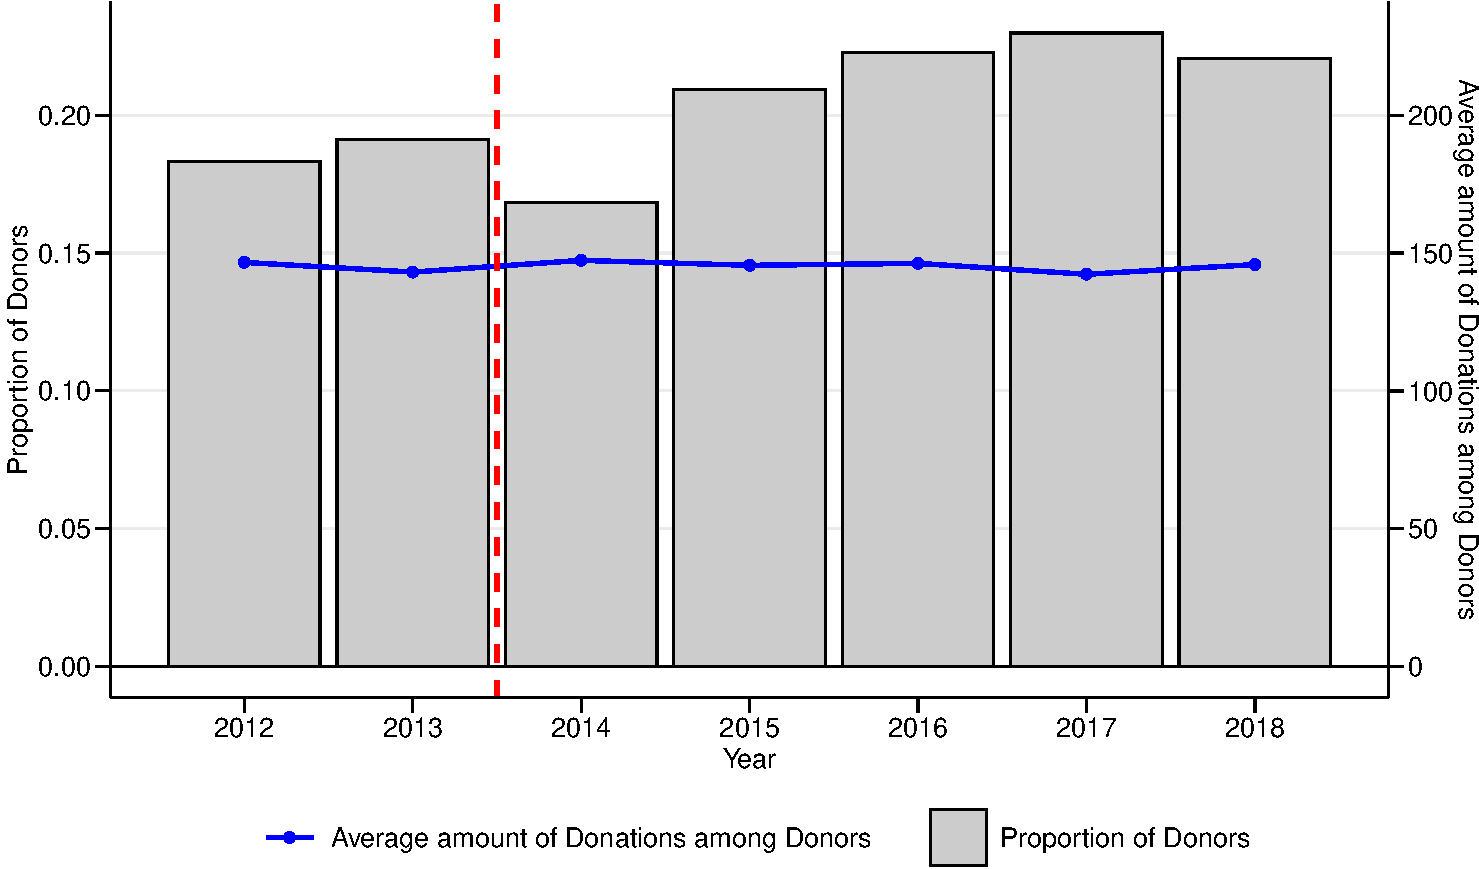
\includegraphics[width=0.85\linewidth,]{C:/Users/katoo/Desktop/NASTAB/paper/draft_files/figure-latex/SummaryOutcome-1} 

}

\caption{Proportion of Donors and Average Donations among Donors. Notes: The left and right axises measure prooortion of donors and the average amount of donations among donors, respectively. Authors made this graph based on NaSTaB data.}\label{fig:SummaryOutcome}
\end{figure}

Table \ref{tab:SummaryCovariate}
shows summary statistics of our data.\footnote{Respondents answer the amount of donation for seven specific purposes last year. Seven specific purposes are policitical parties, educational organizations, social welfare organizations, organizations for culutre and art, religious groups, charity activies organaized by religious group, other purposes. We sum up the amount of donations, and consider it as the annual charitable giving.}
The first panel of this table shows variables about charitable giving.
The NaSTaB asks respondents to answer the amount of donation last year.
This is the first outcome variables.
Using this, we make a dummy taking 1 if respondent donated last year.
This is the second outcome variables to
estimate the price effect on the decision of donations.
This table shows that
the average amount of donation is almost 300,000 KRW (300 USD),
and the proportion of donors is roughly 20\%.
Figure \ref{fig:SummaryOutcome} shows the time-series of two variables.
The blue line shows the average amount of donation among donors.
In each year, its value is nearly 1.5 million KRW (1,500 USD),
which is 7\% of average annual taxable income.
The gray bar shows the proportion of donors.
After the tax reform, the proportion of donors decreases
by 2 percentage points.
After that, the proportion of donors is greter than 20\%.

\begin{figure}[t]

{\centering 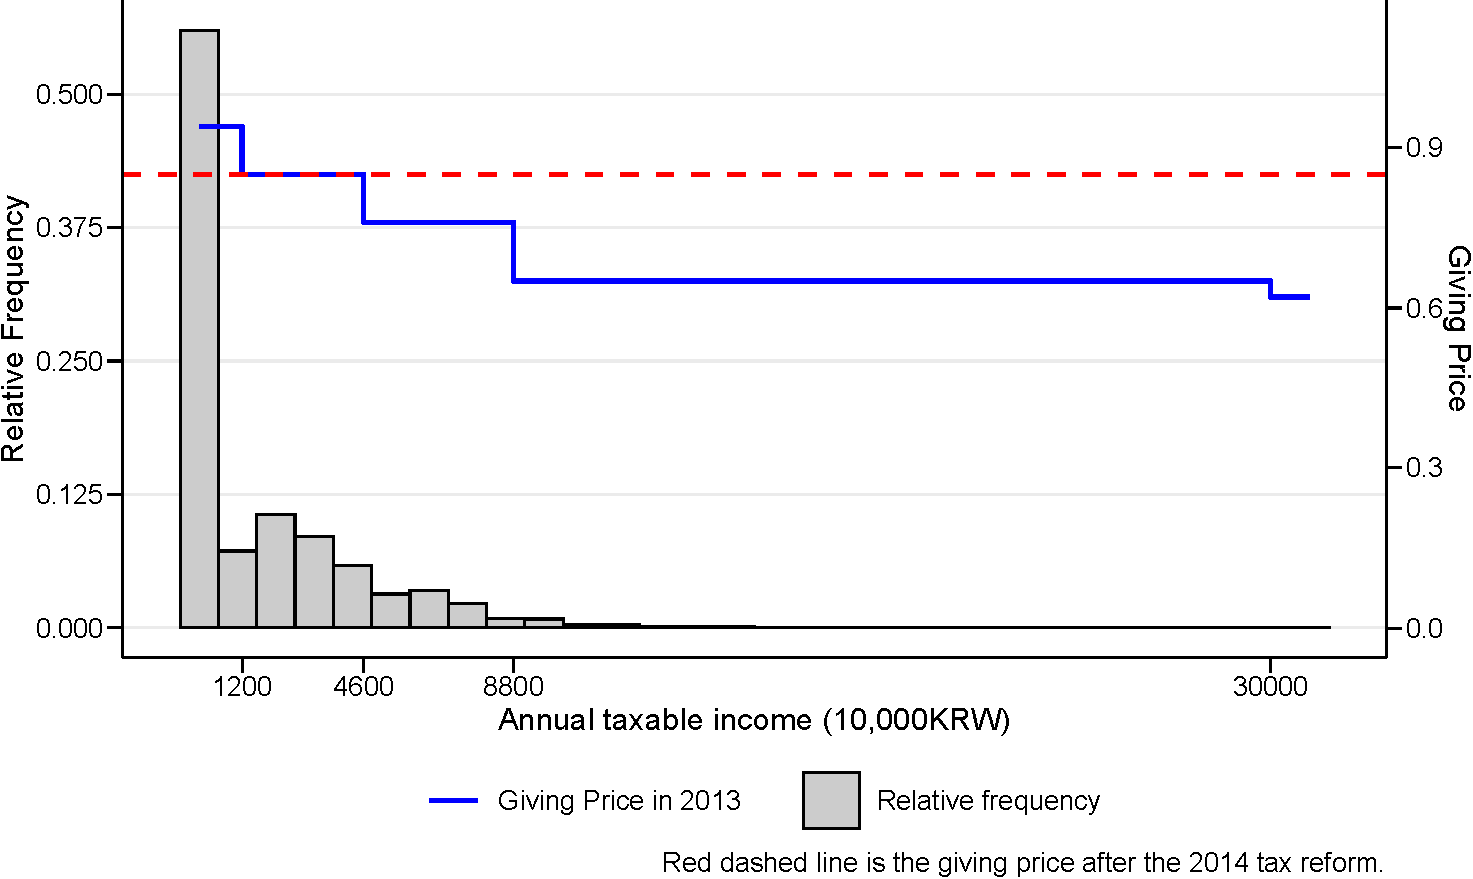
\includegraphics[width=0.85\linewidth,]{C:/Users/katoo/Desktop/NASTAB/paper/draft_files/figure-latex/SummaryPrice-1} 

}

\caption{Income Distribution and Relative Giving Price in 2013. Notes: The left and right axis measure the relative frequency of respondents and the relative giving price, respectively. A blue step line and a red dashed horizontal line represents the giving price in 2013 and 2014, respectively. The grey bar shows income distribution in 2013.}\label{fig:SummaryPrice}
\end{figure}

The second panel of Table \ref{tab:SummaryCovariate}
shows variables about income, tax report, and the giving price.
NaSTaB asks respondents to answer the annual labor income last year.
In our sample,
the average annual taxable income is 18.76 million KRW (18,760 USD).
According to the National Tax Statistical Yearbook
published by Korean National Tax Service,
the average annual taxable income is
32.77 million (32,770 USD) from 2012 to 2018
for employees who submitted the tax return.
Since our sample includes subjects with no labor income, such as housewives,
our sample mean of income is lower than
the average income calculated by the public organizations.
In Figure \ref{fig:SummaryPrice},
the gray bars show the distribution of annual taxable income in 2013.
The income distribution is right-skewed.

Using this variable,
we construct the giving price
under the tax deduction system (2012 and 2013).\footnote{The giving price shown in Table \ref{tab:SummaryCovariate} is the \emph{first} giving price. The giving price can be manipulated by an amount of donation. To avoid this endogeneity, we use the giving price where the amount of donation is zero. We will discuss this issue in the next section.}
After the tax reform (after 2014),
the giving price is 0.85 regardless of labor income,
as we explained in Section \ref{taxreform}.
In Figure \ref{fig:SummaryPrice},
the blue line shows the giving price in 2012 and 2013,
while the red dashed line shows the giving price after 2014.
From this figure,
those whose annual income is less than 120,000,000 KRW
(120,000 USD) in 2013 could receive benefit from the 2014 tax reform
because the tax reform decreases the giving price.
On the other hand,
those whose annual income is greater than
460,000,000 KRW (460,000 USD) in 2013 had a loss by the 2014 tax reform
since the tax reform increases the giving price.

\begin{figure}[t]

{\centering 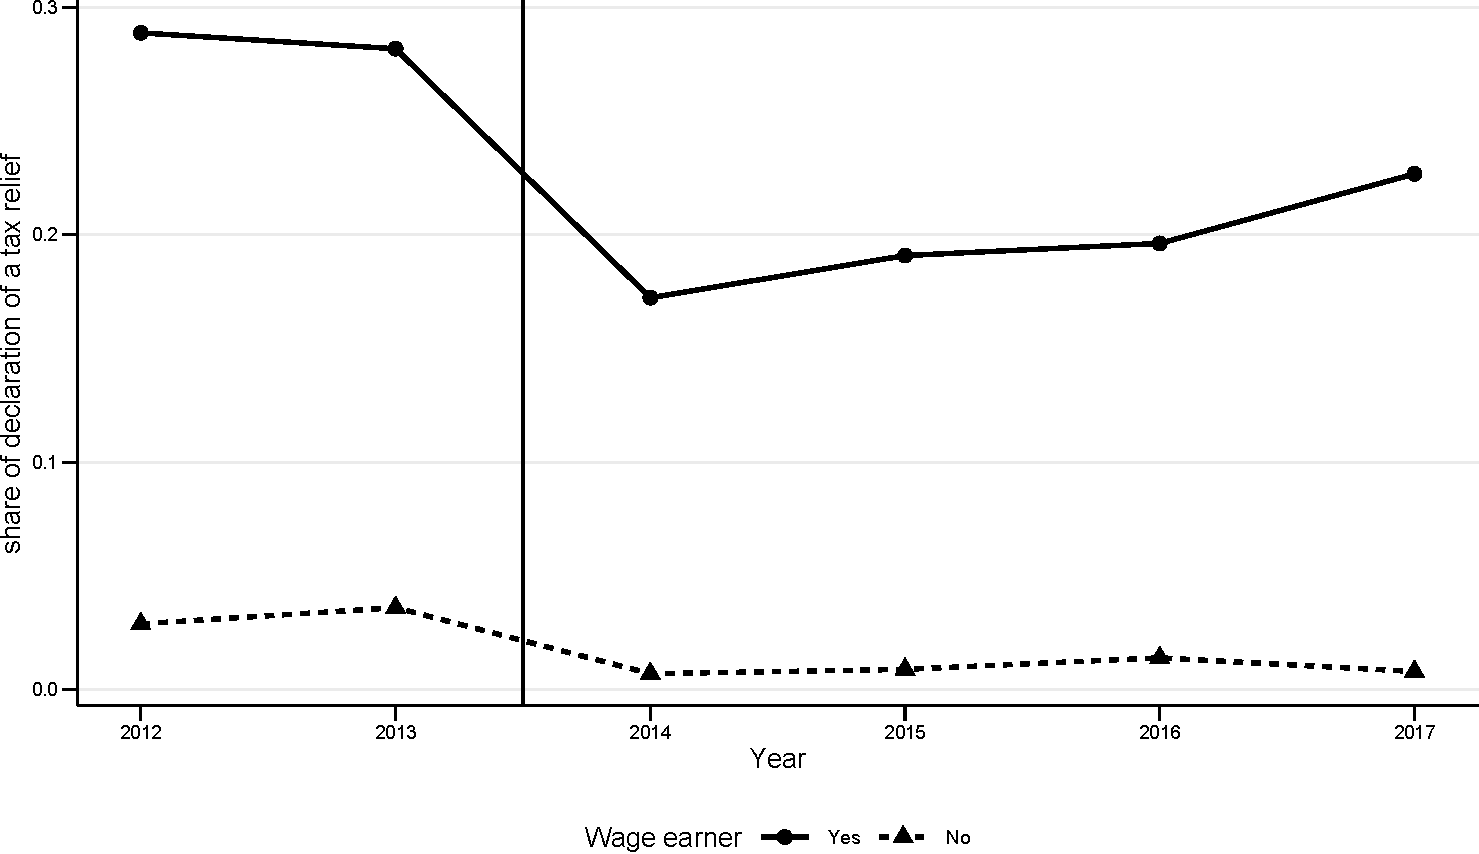
\includegraphics[width=0.85\linewidth,]{C:/Users/katoo/Desktop/NASTAB/paper/draft_files/figure-latex/SummaryRelief-1} 

}

\caption{Share of Tax Relief. Notes: A solid line is the share of applying for tax relief among wage eaners. A dashed line is the share of applying for tax relief other than wage earners.}\label{fig:SummaryRelief}
\end{figure}

The NaSTaB also asks respondents
to answer whether they declared a tax relief of giving.
This survey data separately asks whether subjects applied for tax
relief on giving via tax filing (this is used for \emph{total} income
(e.g., business income, dividend income and rental income)) or not,
and whether subjects applied for tax reilef on giving via tax withholding
(this is used for \emph{labor} income.).
We make a dummy taking one if subjects applied for either tax relief.
Table \ref{tab:SummaryCovariate} shows
the proportion of declaration is about 11\%.

\hypertarget{statistical-model}{%
\section{Statistical Model}\label{statistical-model}}

\begin{figure}[t]

{\centering 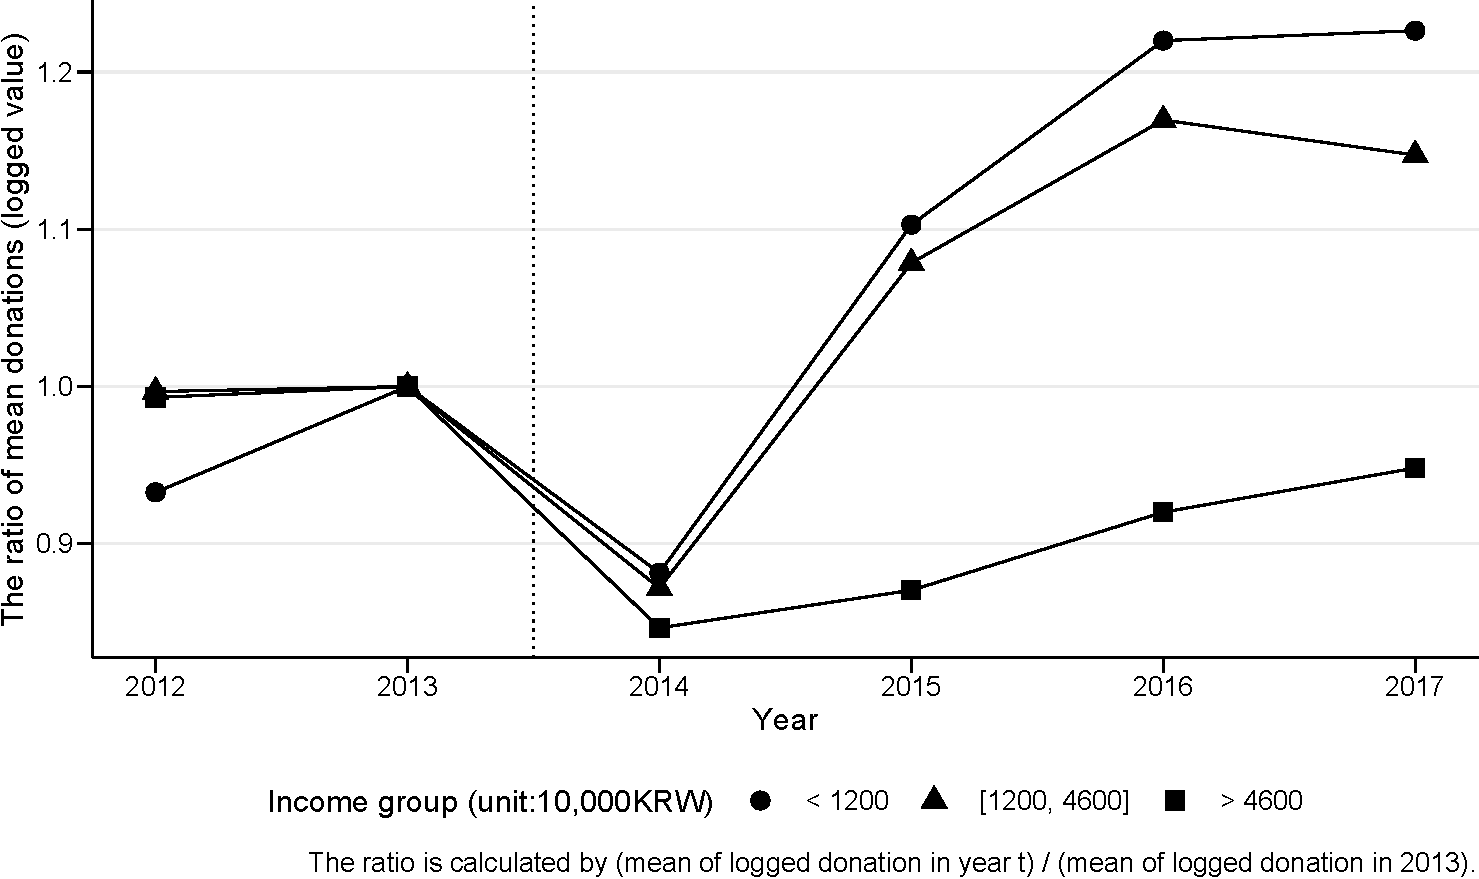
\includegraphics[width=0.85\linewidth,]{C:/Users/katoo/Desktop/NASTAB/paper/draft_files/figure-latex/SummaryOutcome2-1} 

}

\caption{Average Logged Giving in Three Income Groups. Notes: We created three income groups, with the relative price of giving rising (circle), unchanged (triangle), and falling (square) between 2013 and 2014.}\label{fig:SummaryOutcome2}
\end{figure}

To estimate the giving price elasticity,
we use DID-like strategy which exploit the fact that the giving price was unified in 2014
while the price was different for tax payers with different incomes.
Figure \ref{fig:SummaryOutcome2} shows the logarithmic average of donations for each year for the three income groups, which is standardized to be 1 in 2013.
We created three income groups, with the relative price of giving rising (lower than 12,000,000 KRW),
unchanged (between 12,000,000 KRW and 46,000,000 KRW),
and falling (higher than 46,000,000 KRW) between 2013 and 2014.

We can observe two facts from this figure.
First, before the tax reform, the amount of donations of income groups whose prices have increased or unchanged has remained the same,
but since the 2014 tax reform, the amount of giving of income groups whose price has risen was lower than the group whose price has unchanged.
Second, before the tax reform, the income group whose price decreased was lower than the group whose prices did not change,
but after the 2014 tax reform, the average donations of the two groups have been about the same.
In particular, since 2016,
the average donation amount of income groups whose price has decreased is slightly higher than that of groups whose price has not changed.
These facts in descriptive statistics suggest that
the exogenous shock of giving price by the 2014 tax reform has produced a price effect for donations.

Using this exogenous change in price, we estimate the price elasticity of donations.
Then, we assume the following 2-way fixed effect model:
\begin{equation}
    \ln g_{it} = \varepsilon_p R_{it} \ln p_{it}(y_{it}, g_{it}) + \varepsilon_y \ln y_{it} 
    + X_{it}\beta +\mu_i +\iota_t +u_{it}, \label{eq:intensive}
\end{equation}
where \(g_{it}, p_{it}\) and \(y_{it}\) respectively indicates
the amount of giving, the giving price (if they apply for a tax deduction/credit), and income of \(i\) in year \(t\).
\(R_{it}\) is a dummy taking one if individual \(i\) applies for a tax deduction/credit in year \(t\).
If s/he does not apply for a tax deduction/credit (\(R_{it} = 0\)), then the relative giving price is one (\(p_{it} = 1\)),
and its logarithmic value is zero.
\(\mu_i, \iota_t\) and \(u_{it}\) are individual fixed effect, year fixed effect, and the error term, respectively.
\(X_{it}\) is a vector of covariates including square of age, industry dummy, and area dummy.

Our parameter of interest is the price elasticity of giving, denoted by \(\varepsilon_p\).
When estimating this parameter,
we need to address the issue of donation price endogenous
and deduction application endogenous.
In the following subsections, we discuss how to deal with each endogeneity.

\hypertarget{endogenity-of-giving-price-p_it}{%
\subsection{\texorpdfstring{Endogenity of Giving Price \(p_{it}\)}{Endogenity of Giving Price p\_\{it\}}}\label{endogenity-of-giving-price-p_it}}

Our identification strategy is price changes due to the 2014 tax reform.
However, the relative price of donations is endogenous
because it depends on the amount of income and charitable giving under the tax deduction system (before the 2014 tax reform).
To formally show this issue, the relative price of donations \(p_{it}\) is defined as:
\begin{align}
  p_{it}(y_{it}, g_{it}) =
  \begin{cases}
    1 - \tau_t(y_{it} - g_{it})  \quad\text{if}\quad t < 2014  \\
    1 - m \quad\text{if}\quad t \ge 2014
  \end{cases}, \label{eq:price}
\end{align}
where \(\tau_t(\cdot)\) is average tax rate in year \(t\).
As is clear from the above formula,
the (within) variation in giving price depends not only on the 2014 tax reform
but also on the amount of donations and income before 2014,
which are factors in the endogenous nature of the giving price.

In the tax deduction system,
the giving price is endogenous
because taxpayers can reduce the amount of donations and
lower their tax brackets by one level to lower the relative price of giving.
To address this endogeneity, consider the price faced in the first unit of donation denoted by \(p^f_{it}\).
This is called the first-price of giving and is obtained by \(p^f_{it}(y_{it}) = p_{it}(y_{it}, 0)\).
In contrast, \(p_{it}(y_{it}, g_{it})\) is called the last-price of giving.\footnote{Under the tax credit system, the relative price of donations does not depend on the donation amount. Thus, the first-price of giving is equal to the last-price of giving.}
The first-price of giving is unaffected by the manipulation of giving,
so the first-price is exogenous to the donation amount.
Therefore, assuming that the income is exogenous,
we replace \(\ln p_{it}(y_{it}, g_{it})\) in the Equation \eqref{eq:intensive} with \(\ln p^f_{it}(y_{it})\)
to estimate the first-price elasticity of giving.
Also, using the first-price of giving as the instrumental variable for that last-price,
we estimate the Equation \eqref{eq:intensive} with 2SLS with fixed effects.

\hypertarget{endogenity-of-applying-for-tax-relief-r_it}{%
\subsection{\texorpdfstring{Endogenity of Applying for Tax Relief \(R_{it}\)}{Endogenity of Applying for Tax Relief R\_\{it\}}}\label{endogenity-of-applying-for-tax-relief-r_it}}

We use instrumental variable method to address the endogeneity caused by self-selection of tax deductions.
If there is no (physical or psychological) cost to declare a tax relief,
then all individuals should declare a tax relief.
However, as shown in Table \ref{tab:SummaryCovariate},
declaring a tax relief may incur some costs because some respondents did not declare a tax relief.
Employment status is one dimension of variation of applied cost.
For the declaration, self-employed workers have to retain the certificate until they submit tax return although wage earners can declare tax relief and submit the certificate through their company at any time.
Figure \ref{fig:SummaryRelief} shows that
the proportion of declaring a tax relief among employees is higher than the others.
Thus, we use the wage earner dummy, denoted by \(\text{WageEarner}_{it}\), as an instrument of a declaration.

The instrumental variable \(\text{WageEarner}_{it}\) must hold independence of \(u_{it}\) conditional on covariates.\footnote{We allow arbitrary correlation between instrument and fixed effects.}
There are two potential sources to violate this assumption.
First, the employment status may produce income variation.
If this is true, then the employment status affects charitable giving through an income effect.
Second, an opportunity of giving may depend on employment status.
For example, a doctor and a public servant may tend to donate than the others.
If so, the instrument is correlated with \(u_{it}\).
Since we control incomes and industry dummies, we can avoid this problem.

We take three approaches using the wage earner dummy as the instrumental variable.
First, we estimate the following outcome equation with 2SLS with fixed effects:
\begin{equation}
    \ln g_{it} = \varepsilon_{pi} (R_{it} \ln p^f_{it}(y_{it})) + \varepsilon_y \ln y_{it} 
    + X_{it}\beta +\mu_i +\iota_t +u_{it}, \label{eq:stage2}
\end{equation}
where \(R_{it} \ln p^f_{it}(y_{it})\) is instrumented by
\(\text{WageEarner}_{it} \times \ln p^f_{it}(y_{it})\).

The remaining two approaches use the propensity score (PS) of tax relief applications.
To get a propensity score,
we implement a probit estimation with the following selection equation:
\begin{equation}
  R_{it} = 1[\delta_0 + Z_{it} \delta_1 + u_{it1} > 0], \label{eq:stage1}
\end{equation}
where \(Z_{it} = (\text{WageEarner}_{it}, \ln p^f_{it}(y_{it}), \ln y_{it}, X_{it})\).

We estimate this model with a full sample (pooled probit model) or
a subsample (separated probit model) divided by year,
and calculate the propensity score by \(P(Z_{it}) = \Phi(\hat{\delta}_0 + Z_{it} \hat{\delta}_1)\)
where \(\Phi(\cdot)\) is the cumulative function of the standard normal distribution.
The latter estimation method allows the two coefficients \((\delta_0, \delta_1)\) to vary over time.
The second approach estimates equation \eqref{eq:stage2} with 2SLS with fixed effects,
using \(P(Z_{it}) \times \ln p^f_{it}(y_{it})\) as the instrumental variable of \(R_{it} \ln p^f_{it}(y_{it})\).
The third approach estimates the following outcome equation by OLS:
\begin{equation}
    \ln g_{it} = \varepsilon_{pi} (P(Z_{it}) \ln p^f_{it}(y_{it})) + \varepsilon_y \ln y_{it} 
    + X_{it}\beta +\mu_i +\iota_t +u_{it}. \label{eq:stage2red}
\end{equation}

\hypertarget{results}{%
\section{Results}\label{results}}

In this section, we report the price elasticity of intensive-margin and
extensive-margin, respectively.
Note that we provide Appendix A with the first-stage estimation results
used to calculate the propensity score.
As a basic result, even if we control covariates such as income,
giving price, and industry dummy,
the wage earner dummy is strongly and positively correlated with
the application of donation deduction/credit.
However, when the sample is divided by year,
the partial correlation between the wage earner dummy and
the application of donation deduction/credit in 2013 is
statistically insignificant.

\hypertarget{intensive-margin}{%
\subsection{Intensive Margin}\label{intensive-margin}}

\begin{table}

\caption{\label{tab:intensive}First-Price Elasticities (Intenstive Margin)}
\centering
\fontsize{9}{11}\selectfont
\begin{threeparttable}
\begin{tabular}[t]{lccccc}
\toprule
\multicolumn{1}{c}{ } & \multicolumn{3}{c}{FE-2SLS} & \multicolumn{2}{c}{OLS} \\
\cmidrule(l{3pt}r{3pt}){2-4} \cmidrule(l{3pt}r{3pt}){5-6}
  & (1) & (2) & (3) & (4) & (5)\\
\midrule
Applying tax relief x log(first price) & -1.429*** & -1.506*** & -1.598*** &  & \\
 & (0.398) & (0.354) & (0.361) &  & \\
PS of applying tax relief x log(first price) &  &  &  & -1.584*** & -1.564***\\
 &  &  &  & (0.371) & (0.353)\\
log(income) & 1.162 & 1.102 & 1.030 & 1.037 & 1.013\\
 & (1.112) & (1.084) & (1.085) & (1.110) & (1.116)\\
\midrule
Num.Obs. & 7080 & 7080 & 7080 & 7080 & 7080\\
R2 & 0.820 & 0.820 & 0.820 & 0.820 & 0.820\\
R2 Adj. & 0.693 & 0.693 & 0.693 & 0.693 & 0.694\\
FE: area & X & X & X & X & X\\
FE: industry & X & X & X & X & X\\
FE: panelid & X & X & X & X & X\\
FE: year & X & X & X & X & X\\
Square of age & X & X & X & X & X\\
Instrument & Wage earner x Price & PS x Price & PS x Price &  & \\
Method of PS &  & Pool & Separate & Pool & Separate\\
\bottomrule
\end{tabular}
\begin{tablenotes}
\item Notes: $^{*}$ $p < 0.1$, $^{**}$ $p < 0.05$, $^{***}$ $p < 0.01$. Standard errors are clustered at individual level.
\end{tablenotes}
\end{threeparttable}
\end{table}

Table \ref{tab:intensive} shows
the estimation results of price elasticity of intensive-margin.
Model (1) uses the intersection of the wage earner dummy and
the giving (first) price as an instrumental variable.
Models (2) and (3) use
the intersection of the propensity score of application and
the giving (first) price as an instrumental variable.
We use pooled model and separate model to calculate propensity scores,
respectively.
In models (4) and (5), we add the intersection between
the propensity score of application and the giving (first) price
directly to the explanatory variables.
The estimated value varies slightly depending on the estimation method,
but it is about -1.5.
Therefore, a 1\% price reduction will increase the donation amount by 1.5\%.

We performed some analyzes for the robustness of this result.
The regression table is shown in Appendix A,
but we will briefly describe the results.
We show the results of estimating elasticity excluding 2013 and 2014 data
in Table \ref{tab:rob1intensive} of the Appendix A
to eliminate the effects of tax reform announcements.
If individuals are aware of the 2014 tax reform in advance,
those who make the relative price of giving higher (cheaper)
by the reform should increase (decrease) donations before the reform.
Therefore, the price elasticity is under-biased
due to the announcement effect of tax reform.
As a result, as we expected,
the price elasticity ranges from -1.6 to -1.9,
which is a statistically significant result.

Table \ref{tab:rob2intensive} of the Appendix A shows
the estimation results of the last-price elasticity.
Under the income deduction system,
the relative price of giving that an individual
does not face the first price, but the last price.
Therefore, it is more realistic to estimate the elasticity
using the last price.
However, the last price is an endogenous variable
because it depends on the donation amount.
Therefore, 2SLS estimation was performed using the instrumental variables
used in Table \ref{tab:intensive} as the instruments of
the intersection of application dummy and the last price.
As a result, the price elasticity of donations ranges from -1.7 to -2.1,
which is statistically significant.

In addition,
we estimated price elasticity
using a sample limited to those who applied for tax relief.
In this section, we only outline and provide detailed results in Appendix B.
Correcting the bias due to sample selection by
adding the inverse Mills ratio calculated in the model
shown in Table 1 of Appendix A directly to the explanatory variables,
the estimated price elasticity ranges from -1.3 to -1.6,
which is similar to the main result.
We also confirmed that
this result is robust
even if the announcement effect of tax reform is eliminated
and that the last-price elasticity takes a similar value.\footnote{We further perform two further robustness tests on the relative price of giving. First, the first-price depends only on income. Therefore, if income is endogenous, the first-price is also an endogenous variable. To deal with this problem, we estimate the \(k\)-th order difference model. Second, to directly control the dynamic effects of price and income changes on donations, we add lagged and future changes of these variables to the explanatory variables.}

\hypertarget{extensive-margin}{%
\subsection{Extensive Margin}\label{extensive-margin}}

By changing the outcome variable
from the logarithmic value of giving
to a dummy variable that takes one when donated,
we estimate the extensive-margin price elasticity
with a linear probability model.
The estimated price coefficient value
does not directly reflect the price elasticity,
but we can obtain the price elasticity
by dividing the estimated coefficient value
by the average of the outcome variables.
Also, we focus only on the first-price elasticity
since the decision to donate is the same as
the decision to donate the first unit.

\begin{table}

\caption{\label{tab:extensive}First-Price Elasticities (Extenstive Margin)}
\centering
\fontsize{9}{11}\selectfont
\begin{threeparttable}
\begin{tabular}[t]{lccccc}
\toprule
\multicolumn{1}{c}{ } & \multicolumn{3}{c}{FE-2SLS} & \multicolumn{2}{c}{OLS} \\
\cmidrule(l{3pt}r{3pt}){2-4} \cmidrule(l{3pt}r{3pt}){5-6}
  & (1) & (2) & (3) & (4) & (5)\\
\midrule
Applying tax relief x log(first price) & -0.445*** & -0.509*** & -0.710*** &  & \\
 & (0.172) & (0.124) & (0.113) &  & \\
PS of applying tax relief x log(first price) &  &  &  & -0.416*** & -0.546***\\
 &  &  &  & (0.111) & (0.097)\\
log(income) & 2.105*** & 2.074*** & 1.975*** & 1.955*** & 1.832***\\
 & (0.280) & (0.263) & (0.257) & (0.281) & (0.279)\\
\midrule
Implied price elasticity & -1.863*** & -2.129*** & -2.975*** & -1.743*** & -2.286***\\
 & (0.721) & (0.518) & (0.475) & (0.465) & (0.407)\\
Num.Obs. & 26922 & 26922 & 26922 & 26922 & 26922\\
R2 & 0.679 & 0.681 & 0.687 & 0.663 & 0.663\\
R2 Adj. & 0.569 & 0.572 & 0.580 & 0.547 & 0.547\\
FE: area & X & X & X & X & X\\
FE: industry & X & X & X & X & X\\
FE: panelid & X & X & X & X & X\\
FE: year & X & X & X & X & X\\
Square of age & X & X & X & X & X\\
Instrument & Wage earner x Price & PS x Price & PS x Price &  & \\
Method of PS &  & Pool & Separate & Pool & Separate\\
\bottomrule
\end{tabular}
\begin{tablenotes}
\item Notes: $^{*}$ $p < 0.1$, $^{**}$ $p < 0.05$, $^{***}$ $p < 0.01$. Standard errors are clustered at individual level. Implied price elasticity is obtained by the ratio of estimated coefficient value to share of donors.
\end{tablenotes}
\end{threeparttable}
\end{table}

Table \ref{tab:extensive} shows
the estimation results of extensive-margin price elasticity.
Similar to Table \ref{tab:intensive},
model (1) uses the intersection of the wage earner dummy and
giving price as an instrumental variable.
Models (2) and (3) use the intersection of propensity score of application
and giving price as an instrumental variable.
Models (4) and (5) use OLS to estimate a model that
uses the intersection of propensity score of application and
giving price as an explanatory variable.

As a result, the estimated coefficients are in the range of -0.41 to -0.54.
The extensive-margin price elasticity,
obtained by dividing estimates by the percentage of donors,
ranges from -1.74 to -2.98.
In other words,
a 1\% reduction in relative price due to tax incentives increases
the probability of donation by 1.74\% to 2.98\%.
This result is robust against
the effects of the 2014 tax reform announcement
(See Table \ref{tab:robextensive} in Appendix A,
which shows the results of the same exercise
using subsamples that exclude 2013 and 2014 data).
Therefore,
those who apply for tax relief are sensitive to tax incentives
when deciding on how much to donate rather than whether or not to donate.

\hypertarget{conclusions}{%
\section{Conclusions}\label{conclusions}}

In this paper, we investigate the giving price elasticity using South Korean panel data. As a result, we obtain the following findings.

Firstly, our baseline estimation shows that the giving price elasticity in Korea is less than -1.4 even if we take into account declaration cost of charitable giving. Since the literature of the tax expenditure for charitable giving suggests that the price elasticity is around -1, the result suggests that the impact of declaration cost may be big.

Secondly, we find that. compared to the baseline result, the estimated price elasticity using the data limited to tax filers takes -1.3 \(\sim\) -1.6, which is similar values to the estimated elasticity in the extant research. It implies that the usage of tax return data leads to smaller price elasticity in terms of absolute value.

From the results, we firstly show the giving price elasticity in Korea. However, many things to be considered are remaining. To understand the giving behavior and to contribute the policy making, more sophisticated research is needed.

\newpage

\hypertarget{references}{%
\section*{References}\label{references}}
\addcontentsline{toc}{section}{References}

\hypertarget{refs}{}
\begin{CSLReferences}{1}{0}
\leavevmode\vadjust pre{\hypertarget{ref-Almunia2020}{}}%
Almunia, M., Guceri, I., Lockwood, B., Scharf, K., 2020. More giving or more givers? The effects of tax incentives on charitable donations in the UK. Journal of Public Economics 183. doi:\href{https://doi.org/10.1016/j.jpubeco.2019.104114}{10.1016/j.jpubeco.2019.104114}

\leavevmode\vadjust pre{\hypertarget{ref-Auten2002}{}}%
Auten, G.E., Sieg, H., Clotfelter, C.T., 2002. \href{http://www.jstor.org/stable/3083340}{Charitable giving, income, and taxes: An analysis of panel data}. American Economic Review 92, 371--382.

\leavevmode\vadjust pre{\hypertarget{ref-Backus2019}{}}%
Backus, P.G., Grant, N.L., 2019. How sensitive is the average taxpayer to changes in the tax-price of giving? International Tax and Public Finance 26, 317--356. doi:\href{https://doi.org/10.1007/s10797-018-9500-9}{10.1007/s10797-018-9500-9}

\leavevmode\vadjust pre{\hypertarget{ref-Bakija2011}{}}%
Bakija, J., Heim, B.T., 2011. How does charitable giving respond to incentives and income? New estimates from panel data. National Tax Journal 64, 615--650. doi:\href{https://doi.org/10.17310/ntj.2011.2S.08}{10.17310/ntj.2011.2S.08}

\leavevmode\vadjust pre{\hypertarget{ref-Fack2010}{}}%
Fack, G., Landais, C., 2010. Are tax incentives for charitable giving efficient? Evidence from france. American Economic Journal - Economic Policy 2, 117--141. doi:\href{https://doi.org/10.1257/pol.2.2.117}{10.1257/pol.2.2.117}

\leavevmode\vadjust pre{\hypertarget{ref-Randolph1995}{}}%
Randolph, W.C., 1995. Dynamic income, progressive taxes, and the timing of charitable contributions. Journal of Political Economy 103, 709--738. doi:\href{https://doi.org/10.1086/262000}{10.1086/262000}

\leavevmode\vadjust pre{\hypertarget{ref-Rehavi2013}{}}%
Rehavi, M., Shack, D., 2013. Partial reporting: An example from charitable giving. Working paper of University of British Columbia.

\leavevmode\vadjust pre{\hypertarget{ref-Saez2004}{}}%
Saez, E., 2004. The optimal treatment of tax expenditures. Journal of Public Economics 88, 2657--2684. doi:\href{https://doi.org/10.1016/j.jpubeco.2003.09.004}{10.1016/j.jpubeco.2003.09.004}

\end{CSLReferences}

\newpage

\hypertarget{appendix-appendix}{%
\appendix}


\hypertarget{appendix}{%
\section*{Appendix}\label{appendix}}
\addcontentsline{toc}{section}{Appendix}

\hypertarget{additional-figures-and-tables}{%
\section{Additional Figures and Tables}\label{additional-figures-and-tables}}

\begin{table}[H]

\caption{\label{tab:stage1}Probit Estimation of Selection Equation}
\centering
\fontsize{9}{11}\selectfont
\begin{threeparttable}
\begin{tabular}[t]{lccccccc}
\toprule
\multicolumn{2}{c}{ } & \multicolumn{6}{c}{Separated Probit Model} \\
\cmidrule(l{3pt}r{3pt}){3-8}
  & Pooled & 2012 & 2013 & 2014 & 2015 & 2016 & 2017\\
\midrule
(Intercept) & -212.784 & -195.672*** & -181.767 & -219.403*** & -228.677*** & -209.380*** & -241.117***\\
 & (235.327) & (34.012) & (238.432) & (15.571) & (73.558) & (78.437) & (13.704)\\
1 = Wage earner & 0.426*** & 0.412*** & 0.215** & 0.603*** & 0.534*** & 0.430*** & 0.800***\\
 & (0.041) & (0.095) & (0.094) & (0.132) & (0.122) & (0.106) & (0.129)\\
log(first giving price) & -1.274*** & -1.276 & -2.167** &  &  &  & \\
 & (0.248) & (0.883) & (0.868) &  &  &  & \\
log(income) & 17.905*** & 16.730*** & 15.219*** & 18.930*** & 19.304*** & 17.638*** & 20.643***\\
 & (0.541) & (2.958) & (2.896) & (1.349) & (1.263) & (1.206) & (1.190)\\
Square of age & -0.002 & -0.002 & -0.001 & -0.002 & -0.007* & 0.000 & 0.003\\
 & (0.001) & (0.003) & (0.003) & (0.004) & (0.004) & (0.003) & (0.003)\\
\midrule
Num.Obs. & 26922 & 4261 & 4391 & 4383 & 4550 & 4611 & 4726\\
Log.Lik. & -7660.954 & -1391.073 & -1441.344 & -981.075 & -1118.238 & -1183.661 & -1275.369\\
Std. Errors & Standard & Standard & Standard & Standard & Standard & Standard & Standard\\
Dummy of area & X & X & X & X & X & X & X\\
Dummy of industry & X & X & X & X & X & X & X\\
\bottomrule
\end{tabular}
\begin{tablenotes}
\item Notes: $^{*}$ $p < 0.1$, $^{**}$ $p < 0.05$, $^{***}$ $p < 0.01$.
\end{tablenotes}
\end{threeparttable}
\end{table}

\begin{table}

\caption{\label{tab:rob1intensive}Robustness of First-Price Elasticities (Intenstive Margin)}
\centering
\fontsize{9}{11}\selectfont
\begin{threeparttable}
\begin{tabular}[t]{lccccc}
\toprule
\multicolumn{1}{c}{ } & \multicolumn{3}{c}{FE-2SLS} & \multicolumn{2}{c}{OLS} \\
\cmidrule(l{3pt}r{3pt}){2-4} \cmidrule(l{3pt}r{3pt}){5-6}
  & (1) & (2) & (3) & (4) & (5)\\
\midrule
Applying tax relief x log(first price) & -1.703*** & -1.626*** & -1.673*** &  & \\
 & (0.587) & (0.468) & (0.483) &  & \\
PS of applying tax relief x log(first price) &  &  &  & -1.927*** & -1.857***\\
 &  &  &  & (0.561) & (0.540)\\
log(income) & -0.326 & -0.287 & -0.311 & -0.813 & -0.764\\
 & (1.417) & (1.401) & (1.397) & (1.458) & (1.453)\\
\midrule
Num.Obs. & 4908 & 4908 & 4908 & 4908 & 4908\\
R2 & 0.851 & 0.851 & 0.851 & 0.852 & 0.852\\
R2 Adj. & 0.685 & 0.685 & 0.685 & 0.686 & 0.686\\
FE: area & X & X & X & X & X\\
FE: industry & X & X & X & X & X\\
FE: panelid & X & X & X & X & X\\
FE: year & X & X & X & X & X\\
Square of age & X & X & X & X & X\\
Instrument & Wage earner x Price & PS x Price & PS x Price &  & \\
Method of PS &  & Pool & Separate & Pool & Separate\\
\bottomrule
\end{tabular}
\begin{tablenotes}
\item Notes: $^{*}$ $p < 0.1$, $^{**}$ $p < 0.05$, $^{***}$ $p < 0.01$. Standard errors are clustered at individual level.
\end{tablenotes}
\end{threeparttable}
\end{table}

\begin{table}

\caption{\label{tab:rob2intensive}Last-Price Elasticities (Intensive Margin)}
\centering
\fontsize{9}{11}\selectfont
\begin{threeparttable}
\begin{tabular}[t]{lccc}
\toprule
  & (1) & (2) & (3)\\
\midrule
Applying tax relief x log(last price) & -1.627*** & -1.781*** & -1.901***\\
 & (0.527) & (0.448) & (0.458)\\
log(income) & 1.012 & 0.899 & 0.812\\
 & (1.175) & (1.141) & (1.142)\\
\midrule
Num.Obs. & 6492 & 6492 & 6492\\
R2 & 0.820 & 0.820 & 0.820\\
R2 Adj. & 0.688 & 0.688 & 0.687\\
FE: area & X & X & X\\
FE: industry & X & X & X\\
FE: panelid & X & X & X\\
FE: year & X & X & X\\
Square of age & X & X & X\\
Instrument & Wage earner x Price & PS x Price & PS x Price\\
Method of PS &  & Pool & Separate\\
\bottomrule
\end{tabular}
\begin{tablenotes}
\item Notes: $^{*}$ $p < 0.1$, $^{**}$ $p < 0.05$, $^{***}$ $p < 0.01$. Standard errors are clustered at individual level.
\end{tablenotes}
\end{threeparttable}
\end{table}

\begin{table}

\caption{\label{tab:robextensive}Robustness of First-Price Elasticities (Extenstive Margin)}
\centering
\fontsize{9}{11}\selectfont
\begin{threeparttable}
\begin{tabular}[t]{lccccc}
\toprule
\multicolumn{1}{c}{ } & \multicolumn{3}{c}{FE-2SLS} & \multicolumn{2}{c}{OLS} \\
\cmidrule(l{3pt}r{3pt}){2-4} \cmidrule(l{3pt}r{3pt}){5-6}
  & (1) & (2) & (3) & (4) & (5)\\
\midrule
Applying tax relief x log(first price) & -0.203 & -0.505*** & -0.704*** &  & \\
 & (0.257) & (0.170) & (0.159) &  & \\
PS of applying tax relief x log(first price) &  &  &  & -0.430*** & -0.562***\\
 &  &  &  & (0.162) & (0.145)\\
log(income) & 2.233*** & 2.108*** & 2.026*** & 1.934*** & 1.814***\\
 & (0.322) & (0.298) & (0.293) & (0.331) & (0.328)\\
\midrule
Implied price elasticity & -0.850 & -2.116*** & -2.949*** & -1.801*** & -2.353***\\
 & (1.075) & (0.711) & (0.666) & (0.677) & (0.606)\\
Num.Obs. & 18148 & 18148 & 18148 & 18148 & 18148\\
R2 & 0.716 & 0.725 & 0.730 & 0.709 & 0.710\\
R2 Adj. & 0.553 & 0.567 & 0.576 & 0.543 & 0.543\\
FE: area & X & X & X & X & X\\
FE: industry & X & X & X & X & X\\
FE: panelid & X & X & X & X & X\\
FE: year & X & X & X & X & X\\
Square of age & X & X & X & X & X\\
Instrument & Wage earner x Price & PS x Price & PS x Price &  & \\
Method of PS &  & Pool & Separate & Pool & Separate\\
\bottomrule
\end{tabular}
\begin{tablenotes}
\item Notes: $^{*}$ $p < 0.1$, $^{**}$ $p < 0.05$, $^{***}$ $p < 0.01$. Standard errors are clustered at individual level. Implied price elasticity is obtained by the ratio of estimated coefficient value to share of donors.
\end{tablenotes}
\end{threeparttable}
\end{table}

\clearpage

\hypertarget{estimate-elasiticity-using-subsample}{%
\section{Estimate Elasiticity Using Subsample}\label{estimate-elasiticity-using-subsample}}

\hypertarget{sample-selection-bias-correction}{%
\subsection{Sample Selection Bias Correction}\label{sample-selection-bias-correction}}

This supplement estimates price elasticity
using data from only those who have applied for tax relief.
If there is both
a year in which the same individual applied for tax relief
and a year when it did not,
we use only the year when the person applied for the relief.

Since deduction applications are endogenous as described in this paper,
subsample estimation involves a sample selection bias.
To formally demonstrate this bias, consider the following model:
\begin{align}
  &Y_{it} = \beta  X_{it} + \mu_{i1} + \lambda_{t1} + e_{it1}, \\
  &R_{it} = 1[\gamma_1 Z_{it} + \gamma_2 X_{it} + \mu_{i2} + \lambda_{t2} + e_{it2} > 0].
\end{align}
where \(Y_{it}\) is the logged value of giving amount (\(\ln g_{it}\)),
\(X_{it}\) is the logged value of first giving price (\(\ln p^f(y_{it})\)),
and \(R_{it}\) is the application dummy.
Thus, \(\beta\) represents the price elasticity of giving,
which is our parameter of interest.
\(Z_{it}\) is the wage earner dummy,
an instrument that allows arbitrary corrleation
with \(\mu_{i1}\) and \(\lambda_{i1}\) but
holds that exogeneity with respect to \(u_{i1}\).
\(\mu_i\) and \(\eta_t\) is individual and time fixed effect, respectively.
\(e_{it}\) is error term.
Assume that \(E(e_{it1} |Z_{it}, X_{it}, \mu_{i1}, \lambda_{i1}) = 0\).
Note that, to clarify the problem,
we intentionally do not model covariates such as income.

Since we estimate the model only for those who applied for the deduction,
the conditional expectation of the outcome equation is as follows:
\begin{align}
  E(Y_{it} |Z_{it}, X_{it}, \mu_{i1}, \lambda_{i1}, R_{it} = 1)
  = \beta  X_{it} + \mu_{i1} + \lambda_{t1}
  + E(e_{it1} |Z_{it}, X_{it}, \mu_{i1}, \lambda_{i1}, R_{it} = 1).
\end{align}

The fixed effect estimator of \(\beta\) is unbiased only if
\(E(e_{it1} |Z_{it}, X_{it}, \mu_{i1}, \lambda_{i1}, R_{it} = 1) = 0\).
However, it is difficult to assume that
the idiosyncratic error of the donation amount
is independent of the tax deduction application
due to the simultaneous determination of
the tax deduction application and the donation amount.
Therefore, using the control function approach,
we eliminate this selection bias.

This approach makes the following assumptions
about the error term of the outcome variable:
\begin{align}
  E(e_{it1} | Z_{it}, X_{it}, \mu_{i1}, \lambda_{t1}, e_{it2})
  = E(e_{it1} | e_{it2}) = \rho e_{it2}.
\end{align}
This equation suggests two assumptions.
First, the two fixed effects, \(\mu_{i1}\) and \(\lambda_{t1}\),
and observables, \((X_{it}, Z_{it})\) are independent of
the two error terms, \((e_{it1}, e_{it2})\).
Second, \(e_{it1}\) is linearly correlated with \(e_{it2}\),
the degree of which is constant with respect to time.

Under this assumption,
we can write the conditional expectation of the error term, \(e_{it1}\),
as follows:
\begin{align}
  E(e_{it1} | Z_{it}, X_{it}, \mu_{i1}, \lambda_{t1}, R_{it} = 1)
  = \rho E(e_{it2} | Z_{it}, X_{it}, R_{it} = 1).
\end{align}
Thus, the estimation model that eliminates the selection bias is as follows:
\begin{align}
  Y_{it} = \beta  X_{it} + \mu_{i1} + \lambda_{t1}
  + \rho E(e_{it2} | Z_{it}, X_{it}, R_{it} = 1) + u_{it1},
\end{align}
where, by construction, \(E(u_{it1} | Z_{it}, X_{it}, R_{it} = 1) = 0\).
If we knew \(E(e_{it2} | Z_{it}, X_{it}, R_{it} = 1)\),
then we can obtaine unbiased estimator of \(\beta\).
The correction term \(E(e_{it2} | Z_{it}, X_{it}, R_{it} = 1)\)
can be obtained by the inverse Mills ratio.
To calculate the inverse Mills ratio, we use the probit estimation shown in
\ref{tab:stage1} in Appendix A (pooled model and separate model).

\hypertarget{results-1}{%
\subsection{Results}\label{results-1}}

\begin{table}

\caption{\label{tab:benchmark}First Price Intensive-Margin Elasiticity (Subsample Analysis)}
\centering
\fontsize{9}{11}\selectfont
\begin{tabular}[t]{lccccc}
\toprule
  & (1) & (2) & (3) & (4) & (5)\\
\midrule
log(first price) & -1.325*** & -1.603*** & -1.437*** & -1.304*** & -1.501***\\
 & (0.386) & (0.422) & (0.522) & (0.384) & (0.542)\\
log(annual taxable income) & 2.030 & 4.814** & 4.898** & 1.575 & 1.554\\
 & (1.515) & (2.333) & (2.355) & (1.863) & (1.857)\\
log(first price) x IMR &  &  & -0.254 &  & 0.333\\
 &  &  & (0.645) &  & (0.714)\\
IMR &  & 0.320 & 0.286 & -0.044 & 0.012\\
 &  & (0.202) & (0.186) & (0.137) & (0.183)\\
\midrule
Num.Obs. & 3646 & 3643 & 3643 & 3643 & 3643\\
R2 Adj. & 0.726 & 0.726 & 0.726 & 0.725 & 0.725\\
FE: area & X & X & X & X & X\\
FE: industry & X & X & X & X & X\\
FE: panelid & X & X & X & X & X\\
FE: year & X & X & X & X & X\\
Square age & X & X & X & X & X\\
Method of IMR &  & Pooled & Pooled & Separate & Separate\\
\bottomrule
\end{tabular}
\end{table}

Table \ref{tab:benchmark} shows the estimation results of price elasticity.
Model (1) does not add a selection correction term,
while models (2) and (4) add it to the explanatory variables.
We obtain the inverse mills ratio from the pooled probit model
and the separated probit model, respectively.
Since the coefficient of the correction term is statistically insignificant,
the selection bias of the application of tax relief is not severe.
Therefore, the estimated elasticity is in the range of -1.3 to -1.6
with or without the correction term.
The estimated value is very close to the result of this paper.

Models (3) and (5) considered
the heterogeneity of price elasticity among individuals.
Based on the model in the previous subsection,
we can write a (correlated) random coefficient model
that allows this heterogeneity as follows:
\begin{align}
  Y_{it} = \bar{\beta} X_{it} + \mu_{i1} + \lambda_{t1}
  + \rho E(e_{it2} | Z_{it}, X_{it}, R_{it} = 1)
  + \{(\beta_i - \bar{\beta}) X_{it} +  u_{it1}\},
\end{align}
where \(\bar{\beta} = E(\beta_i | R_i = 1)\).
Then, since \((\beta_i - \bar{\beta}) X_{it}\) is included in the error term,
we cannot obtain unbiased estimator of \(\bar{\beta}\),
which is a parameter of our interest,
by controlling only the selection correction term.

Wooldridge (2015) proposes an estimation method that solves this problem
by making the following assumptions in the elements of this new error term:
\begin{align}
  E(\beta_i - \bar{\beta} | Z_{it}, X_{it}, \mu_{i1}, \lambda_{t1}, e_{it2})
  = E(\beta_i - \bar{\beta} | e_{it2}) = \eta e_{it2}.
\end{align}
Thus, the estimation model that eliminates both the selection bias and
the bias from random coefficient is as follows:
\begin{align}
  Y_{it} =& \beta  X_{it} + \mu_{i1} + \lambda_{t1} \\
  &+ \rho \lambda(Z_{it}, X_{it}) + \eta \lambda(Z_{it}, X_{it}) \times X_{it}
  + \tilde{u}_{it1},
\end{align}
where \(\lambda(Z_{it}, X_{it})\) is the inverse Mills ratio.
Note that \(E(\tilde{u}_{it1} | Z_{it}, X_{it}, R_{it} = 1) = 0\)
by construction.
Therefore,
by simply adding an intersection
between the correction term and the giving price to models (3) and (4),
we can eliminate the bias resulting from the heterogeneous elasticity
and estimate the unbiased average elasticity.

The average elasticity estimated by models (3) and (5) is about -1.5,
which is consistent with the results of this paper.
Also, since the coefficients of the intersection term
between the correction term and the giving price
are statistically insignificant,
the price elasticity is unlikely to vary significantly among individuals.

\begin{table}

\caption{\label{tab:robustbenchmark1}First Price Intensive-Margin Elasiticity without Annoucment Effect (Subsample Analysis)}
\centering
\fontsize{9}{11}\selectfont
\begin{tabular}[t]{lccccc}
\toprule
  & (1) & (2) & (3) & (4) & (5)\\
\midrule
log(first price) & -1.451** & -1.296** & -1.203 & -1.406** & -1.457*\\
 & (0.587) & (0.649) & (0.804) & (0.588) & (0.873)\\
log(annual taxable income) & 1.399 & 0.215 & 0.346 & 1.087 & 1.072\\
 & (1.979) & (2.780) & (2.884) & (2.463) & (2.450)\\
log(first price) x IMR &  &  & -0.158 &  & 0.089\\
 &  &  & (1.025) &  & (1.293)\\
IMR &  & -0.122 & -0.135 & -0.024 & -0.010\\
 &  & (0.290) & (0.299) & (0.196) & (0.294)\\
\midrule
Num.Obs. & 2443 & 2441 & 2441 & 2441 & 2441\\
R2 Adj. & 0.732 & 0.733 & 0.733 & 0.733 & 0.733\\
FE: area & X & X & X & X & X\\
FE: industry & X & X & X & X & X\\
FE: panelid & X & X & X & X & X\\
FE: year & X & X & X & X & X\\
Square age & X & X & X & X & X\\
Method of IMR &  & Pooled & Pooled & Separate & Separate\\
\bottomrule
\end{tabular}
\end{table}

\begin{table}

\caption{\label{tab:robustbenchmark2}Last Price Intensive-Margin Elasiticity (Subsample Analysis)}
\centering
\fontsize{9}{11}\selectfont
\begin{tabular}[t]{lccc}
\toprule
  & (1) & (2) & (3)\\
\midrule
log(last price) & -1.454*** & -1.790*** & -1.429***\\
 & (0.446) & (0.500) & (0.443)\\
log(annual taxable income) & 1.914 & 5.181* & 1.489\\
 & (1.528) & (2.765) & (1.878)\\
IMR &  & 0.382 & -0.042\\
 &  & (0.267) & (0.144)\\
\midrule
Num.Obs. & 3539 & 3536 & 3536\\
R2 Adj. & 0.721 & 0.721 & 0.721\\
FE: area & X & X & X\\
FE: industry & X & X & X\\
FE: panelid & X & X & X\\
FE: year & X & X & X\\
Square age & X & X & X\\
Method of IMR &  & Pool & Separate\\
\bottomrule
\end{tabular}
\end{table}

We show the results of the same robustness test as in this paper
in Tables \ref{tab:robustbenchmark1} and \ref{tab:robustbenchmark2}.
To eliminate the announcement effect of the 2014 tax reform,
Table \ref{tab:robustbenchmark1} shows
estimates excluding 2013 and 2014 data.
As a result, the selection bias and
the bias from the heterogeneous elasticity are not large.
Using the inverse mills ratio by the pooled probit model,
the price elasticity is about -1.2.
Given the heterogeneity of elasticity,
this price elasticity is statistically insignificant.
Moreover,
when we use the inverse mills ratio by the separated probit model,
the price elasticity is about -1.4, which is statistically significant.
Table \ref{tab:robustbenchmark2} shows
the estimation results of the last-price elasticity.
As a result, the elasticity is in the range of -1.4 to -1.8,
which is similar to the result shown in this paper.

\begin{table}

\caption{\label{tab:kdiffbenchmark}$k$-th Difference Model with Instrument}
\centering
\resizebox{\linewidth}{!}{
\fontsize{9}{11}\selectfont
\begin{tabular}[t]{lccccccccc}
\toprule
  & (1) & (2) & (3) & (4) & (5) & (6) & (7) & (8) & (9)\\
\midrule
Difference of first price & -1.923* & -0.324 & -0.256 & -2.416*** & -1.004 & -0.936 & -3.987*** & -1.565*** & -1.589***\\
 & (1.101) & (0.682) & (0.663) & (0.915) & (0.645) & (0.636) & (0.745) & (0.592) & (0.557)\\
Difference of annual income & 1.232 & 3.929 & 3.528 & 7.614* & 4.249 & 4.744 & 5.051* & 0.279 & -1.928\\
 & (3.628) & (2.982) & (2.932) & (4.540) & (2.979) & (3.353) & (3.012) & (2.113) & (2.160)\\
IMR &  & 0.086 & 0.031 &  & 0.090 & 0.121 &  & -0.221 & -0.467**\\
 &  & (0.141) & (0.128) &  & (0.149) & (0.184) &  & (0.188) & (0.184)\\
\midrule
Num.Obs. & 3551 & 1700 & 1700 & 3440 & 1134 & 1134 & 3325 & 819 & 819\\
R2 Adj. & 0.022 & -0.005 & -0.006 & 0.030 & -0.014 & -0.014 & 0.032 & 0.017 & 0.022\\
FE: area & X & X & X & X & X & X & X & X & X\\
FE: industry & X & X & X & X & X & X & X & X & X\\
FE: year & X & X & X & X & X & X & X & X & X\\
Difference of square age & X & X & X & X & X & X & X & X & X\\
Lag & 1-year & 1-year & 1-year & 2-year & 2-year & 2-year & 3-year & 3-year & 3-year\\
Method of IMR &  & Pool & Separate &  & Pool & Separate &  & Pool & Separate\\
\bottomrule
\end{tabular}}
\end{table}

\begin{table}

\caption{\label{tab:leadlagbenchmark}First Price Intensive-Margin Elasiticities Including Lead and Lag}
\centering
\fontsize{9}{11}\selectfont
\begin{tabular}[t]{lcc}
\toprule
  & (1) & (2)\\
\midrule
log(first giving price) & -0.235 & -0.377\\
 & (0.872) & (1.191)\\
log(annual taxable income) & -0.200 & 2.353\\
 & (5.532) & (16.995)\\
\midrule
Num.Obs. & 849 & 849\\
R2 Adj. & 0.784 & 0.783\\
FE: area & X & X\\
FE: industry & X & X\\
FE: panelid & X & X\\
FE: year & X & X\\
Square age & X & X\\
\bottomrule
\end{tabular}
\end{table}

In addition to the same robustness test as in this paper,
the results of the other two robustness tests
are shown in Tables \ref{tab:kdiffbenchmark} and \ref{tab:leadlagbenchmark}.
Table \ref{tab:kdiffbenchmark} is an analysis dealing with
the endogeneity of first-price by income manipulation.
Since income is generally endogenous,
the first-price of giving is also an endogenous variable.
Under the income deduction system,
changes in income affect donations through the income effect
and the giving price through marginal tax rates
(Auten et al., 2002; Bakija and Heim, 2011; Randolph, 1995).
Therefore, following Almunia et al. (2020) and Bakija and Heim (2011),
we estimate the following k-th difference model:
\begin{align}
  \Delta^k \ln g_{it} = \varepsilon_p \Delta^k \ln p^f_{it}(y_{it})
  + \varepsilon_y \Delta^k \ln y_{it} + \Delta^k X_{it} \beta
  + \mu_i + \iota_t + v_{it},
\end{align}
where \(\Delta^k \ln g_{it} = \ln (g_{it} / g_{it-k})\),
and \(\Delta^k \ln y_{it} = \ln (y_{it} / y_{it-k})\).
The variable
\(\Delta^k p^f_{it}(y_{it}) = \ln (p^f_{it}(y_{it}) / p^f_{it-k}(y_{it-k}))\)
is instumented by \(\ln (p^f_{it}(y_{it-k})/p^f_{it-k}(y_{it-k}))\).

As a result,
the price elasticity changes greatly
depending on the correction term of the selection,
but the degree of the selection bias is not large.
In addition, when we add the correction term,
the price elasticity is about -1.5 in the 3-year difference model,
which is similar to the result of this paper.
However, in the 1-year difference model and 2-year difference model,
the absolute value of price elasticity is less than 1,
which is statistically insignificant.
Therefore, the value of price elasticity is unstable
for the number of years of lag.

Table \ref{tab:leadlagbenchmark} adds
lagged and future changes of giving price and income
to the explanatory variables
to directly control the dynamic effects of
price and income changes on donations (proposed by Bakija and Heim (2011)).
As a result, price elasticity is statistically insignificant.
However, because our data is unbalanced panel data,
the sample size is quite small.
In that respect, the results of this analysis are unreliable.

\clearpage

\end{document}
